%%% LaTeX Template: Two column article
%%%
%%% Source: http://www.howtotex.com/
%%% Feel free to distribute this template, but please keep to referal to http://www.howtotex.com/ here.
%%% Date: February 2011

%%% Preamble
\documentclass[	DIV=calc,%
							paper=a4,%
							fontsize=12pt,%
							onecolumn]{scrartcl}	 					% KOMA-article class

\usepackage{lipsum}													% Package to create dummy text
\usepackage[brazil]{babel}										% English language/hyphenation
\usepackage[protrusion=true,expansion=true]{microtype}				% Better typography
\usepackage{amsmath,amsfonts,amsthm}					% Math packages
\usepackage[pdftex]{graphicx}									% Enable pdflatex
\usepackage[svgnames]{xcolor}									% Enabling colors by their 'svgnames'
\usepackage[hang, small,labelfont=bf,up,textfont=it,up]{caption}	% Custom captions under/above floats
\usepackage{epstopdf}												% Converts .eps to .pdf
\usepackage{subfig}													% Subfigures
\usepackage{booktabs}												% Nicer tables
\usepackage{fix-cm}													% Custom fontsizes
\usepackage[utf8]{inputenc}
\usepackage[top=2.5cm, bottom=2.5cm, left=2.5cm, right=2.5cm]{geometry}
\usepackage[ddmmyyyy]{datetime}
\addto\captionsenglish{%
	\renewcommand\tablename{Tabela}
	\renewcommand\figurename{Figura}
} 
 

 
%%% Custom sectioning (sectsty package)
\usepackage{sectsty}													% Custom sectioning (see below)
\allsectionsfont{%															% Change font of al section commands
	\usefont{OT1}{phv}{b}{n}%										% bch-b-n: CharterBT-Bold font
	}

\sectionfont{%																% Change font of \section command
	\usefont{OT1}{phv}{b}{n}%										% bch-b-n: CharterBT-Bold font
	}



%%% Headers and footers
\usepackage{fancyhdr}												% Needed to define custom headers/footers
	\pagestyle{fancy}														% Enabling the custom headers/footers
\usepackage{lastpage}	

% Header (empty)
\lhead{}
\chead{}
\rhead{}
% Footer (you may change this to your own needs)

%% ====================================
%% ====================================
%% mude o rodape  do projeto
%% ====================================
%% ====================================

\lfoot{\footnotesize \texttt{JSF - JavaServer Faces} \textbullet ~Tópicos Em Computação}


\cfoot{}
\rfoot{\footnotesize página \thepage\ de \pageref{LastPage}}	% "Page 1 of 2"
\renewcommand{\headrulewidth}{0.0pt}
\renewcommand{\footrulewidth}{0.4pt}



%%% Creating an initial of the very first character of the content
\usepackage{lettrine}
\newcommand{\initial}[1]{%
     \lettrine[lines=3,lhang=0.3,nindent=0em]{
     				\color{DarkGoldenrod}
     				{\textsf{#1}}}{}}



%%% Title, author and date metadata
\usepackage{titling}															% For custom titles

\newcommand{\HorRule}{\color{DarkGoldenrod}%			% Creating a horizontal rule
									  	\rule{\linewidth}{1pt}%
										}

\pretitle{\vspace{-30pt} \begin{flushleft} \HorRule 
				\fontsize{50}{50} \usefont{OT1}{phv}{b}{n} \color{DarkRed} \selectfont 
				}

%% ====================================
%% ====================================
%% mude o titulo  do projeto
%% ====================================
%% ====================================

\title{JSF - JavaServer Faces}					% Title of your article goes here

%% ====================================



\posttitle{\par\end{flushleft}\vskip 0.5em}

\preauthor{\begin{flushleft}
					\large \lineskip 0.5em \usefont{OT1}{phv}{b}{sl} \color{DarkRed}}
\author{Cleverson Tiago Rosa Ramos, Nasser Ruiz Rehman, Rogério Teixeira de Souza }  	% Author name goes here


\postauthor{\footnotesize \usefont{OT1}{phv}{m}{sl} \color{Black} 
					\\Universidade Tecnológica Federal do Paraná - Câmpus Cornélio Procópio 								% Institution of author
					\par\end{flushleft}\HorRule}

\date{}																				% No date




%%% Begin document
\begin{document}
\maketitle
\thispagestyle{fancy} 	
\thispagestyle{empty}		% Enabling the custom headers/footers for the first page 
% The first character should be within \initial{}




%% ====================================
%% ====================================
%% mude o resumo  do projeto
%% ====================================
%% ====================================
%%\initial{E}\textbf{ste modelo deve ser utilizado para entrega de relatório individual e projeto. Coloque aqui o resumo do projeto}

%% ====================================
\begin{figure}
	\centering
	
\includegraphics{utfpr}
\end{figure}

\vspace{3cm}
\centerline{\textit{\textbf{26 de Junho de 2019}}}
%\centerline{\textit{\textbf{\today}}}

\clearpage
    \renewcommand*\listfigurename{Lista de figuras}
\listoffigures






\clearpage
\renewcommand{\contentsname}{Sumário}
\tableofcontents
\clearpage

%% ====================================
%% ====================================
%% Inicio do texto
%% ====================================
%% ====================================
\section{Introdução ao JSF}

JSF significa "JavaServer Faces". O JSF é uma estrutura que permite que desenvolvedores da Web construam interfaces com o usuário para aplicativos JavaServer. É suportado por servidores da Web que executam o Java Enterprise Edition (Java EE).

O JSF simplifica a criação de aplicativos da Web fornecendo um conjunto padrão de ferramentas (ou uma API) para construir interfaces com o usuário. Por exemplo, em vez de codificar um formulário da Web em HTML, um desenvolvedor pode, em vez disso, chamar uma função JSF simples que gera o formulário. Outra função JSF pode ser usada para processar os dados inseridos pelo usuário. Essas funções são processadas no servidor e os dados resultantes são enviados para o navegador do cliente.

O JSF beneficia os desenvolvedores fornecendo objetos reutilizáveis que podem ser facilmente inseridos em páginas da Web. No entanto, esses componentes também são benéficos para os visitantes do site, pois produzem elementos de interface padronizados. Como o código Java é processado no servidor, a aparência dos objetos da Web gerados é consistente em vários sites. Além disso, os componentes do JSF são testados em várias plataformas, portanto funcionam bem em todos os principais navegadores.

Embora o JSF seja frequentemente usado para criar elementos básicos de páginas da Web, ele também oferece suporte a recursos avançados, como acesso ao banco de dados, interação Ajax e ações de página JavaScript. Esses recursos são úteis para criar sites dinâmicos que geram páginas on-the-fly.\\~\\



%\begin{itemize}
	%\item o endereço no github;
%\end{itemize}


\section{Conteúdo}


\subsection{Benefícios}

O JSF reduz o esforço na criação e manutenção de aplicativos, que serão executados em um servidor de aplicativos Java e renderizarão a UI do aplicativo em um cliente de destino. JSF facilita o desenvolvimento de aplicativos da Web:
\begin{itemize}
\item Fornecendo componentes de interface do usuário reutilizáveis;
\item Facilitando a transferência de dados entre os componentes da interface do usuário;
\item Gerenciando o estado da interface do usuário em várias solicitações do servidor;
\item Ativando a implementação de componentes customizados;
\item Conectando o evento do lado do cliente ao código do aplicativo do lado do servidor.
\end{itemize}

\subsection{Modelo de Componente da IU do JSF}

O JSF fornece aos desenvolvedores a capacidade de criar aplicativos da Web a partir de coleções de componentes da interface do usuário que podem se renderizar de maneiras diferente para vários tipos de clientes.

JSF fornece:
\begin{itemize}
\item Biblioteca central;
\item Um conjunto de componentes base da interface do usuário - elementos padrão de entrada HTML;
\item Extensão dos componentes de UI base para criar bibliotecas de componentes de UI adicionais ou para estender componentes existentes;
\item Vários recursos de renderização que permitem que os componentes da UI do JSF se renderizem de maneira diferente, dependendo dos tipos de clientes.
\end{itemize}

\subsection{O que é o padrão de design MVC?}

O padrão de design MVC projeta um aplicativo usando três módulos separados:
\begin{itemize}
\item Model - Carrega dados e login;
\item View - Mostra a interface do usuário;
\item Controller - Manipula o processamento de um aplicativo.
\end{itemize}

O objetivo do padrão de design MVC é separar o modelo e a apresentação, permitindo que os desenvolvedores se concentrem em suas habilidades principais e colaborem de forma mais clara.

Os designers da Web precisam se concentrar apenas na camada de visualização, em vez de na camada de modelo e de controlador. Os desenvolvedores podem alterar o código do modelo e normalmente não precisam alterar a camada de visualização. Os controladores são usados para processar ações do usuário. Nesse processo, o modelo e as visualizações da camada podem ser alterados.

\subsection{Arquitetura JSF}

O aplicativo JSF é semelhante a qualquer outro aplicativo da Web baseado em tecnologia Java [Figura 1].

Ele é executado em um contêiner de servlet Java e contém:
\begin{itemize}
\item Componentes JavaBeans como modelos contendo funcionalidade e dados específicos do aplicativo;
\item Uma biblioteca de tags personalizadas para representar manipuladores e validadores de eventos;
\item Uma biblioteca de tags personalizadas para renderizar componentes da interface do usuário;
\item Componentes de interface do usuário representados como objetos com estado no servidor;
\item Classes auxiliares do lado do servidor;
\item Validadores, manipuladores de eventos e manipuladores de navegação;
\item Arquivo de recursos de configuração do aplicativo para configurar recursos do aplicativo.\\~\\
\end{itemize}


\subsection{Ciclo de Vida}

O ciclo de vida da aplicação JSF consiste em seis fases, que são as seguintes:
\begin{itemize}
\item Fase de visualização de restauração;
\item Aplicar fase de valores de solicitação - eventos de processo;
\item Fase de validação de processos - eventos de processo;
\item Atualize a fase de valores do modelo - eventos de processo;
\item Invocar fase de aplicação - eventos de processo;
\item Fase de resposta de renderização.
\end{itemize}

\section{Conceitos de JSF}


\subsection{Renderers JSF}

O Renderers é a classe, onde ela é designada por renderizar os componentes criados, para que seja visível para os clientes que está utilizando o sistema no lado cliente. Está Classe é especificamente responsável pela codificação e decodificação dos componentes, onde a codificação mostra os componentes e a decodificação pega os valores digitados pelos usuários nos componentes.

Nós dias atuais, com a vasta gama de dispositivos que acessa a internet, os programadores de sistemas têm a incitação em produzir componentes eu possa funcionar em varias plataformas. Como por exemplo, aplicativos funcionando em vários navegadores web e que possa funcionar também em dispositivos moveis. Com o JFS está função acaba se tornando simples, pois os componentes são renderizados separadamente, para que possa ser utilizado em diferentes dispositivos independentemente das resoluções das telas.

Encoding: Por exemplo: suponhamos que usamos a tag h: inputText . 
Portanto, o renderizador do componente associado a essa tag produz a saída conforme [Figura 2].

A página codificada é enviada para o navegador e exibida conforme [Figura 3].

Decoding: Após o cliente preencher e enviar o formulário, conforme mostra a figura 2, o navegador será responsável por mandar estes dados para o servidor. Onde estes dados que estão em cada componetes ficaram salvos em uma tabela Hash e poderá ser acessado e ser interpretados, denominando assim o Decoding.

O controlador da tags de saída html solicita que cada componente seja renderizado. O manipulador de tag chama dois métodos de renderização para cada componente:

encodeBegin () em doStartTag ()    e  encodeEnd () em   doEndTag (). 

\subsection{Managed Bean}

O Managed Bean é a classe responsável de receber os dados de uma View ou página em Xhtml, onde são os dados que o usuário digitou nesta tela ou interação do cliente com a tela e está responsabilidade que designada ao Managed Bean, ou seja, é o Controller de uma aplicação em MVC [Figura 4].

Os Escopos de Maneged Beans JSF podem ser definidos através de anotações do pacote Java.faces.bean. Quando se instancia um objeto da classe do Maneged Bean, ou recuperará uma instancia do namemoria. e Todas as instancias possuem um tempo de vida, que é definido dependendo do escopo usado no Maneged Beans.

Definindo os comportamentos de cada tela e sistemas, onde cada escopo resolve algum tipo especifico de problema e cada um tem uma finalidade.

Os mais importantes são:

\begin{itemize}
\item @NoneScoped: o bean será instanciado a cada vez que for referenciado.
\item @RequestSoped: este é o padrão do JSF, caracteriza-se por ter vida curta, começando quando é referenciado em uma única requisição do protocolo HTTTP e terminando quando a resposta é enviada de volta ao cliente.
\item @ViewScoped: a instancia permanece ativa até que o usuário navegue para a próxima página.
\end{itemize}

SessionScoped: mantem a instancia durante diversas requisições e até mesmo navegações entre páginas, até que a sessão do usuário seja invalidade ou tempo pelo limite de tempo. Cada usuário possui sua sessão de navegação, portanto, os objetos não são compartilhados entre si.

ApplicationScoped: Mantem a instancia dos objetos durante o tempo de execuções das aplicações. E um escopo que compartilha os objetos para todos os usuários do sistema.

\subsection{Bean Validation}

A API de Bean Validation fornece uma facilidade para validar os objetos em diferentes camadas da aplicação. JavaServer Faces integre com esta tecnologia para validar objetos preenchidos pelas páginas Web.

A vantagem de se usar o Bean Validation é que as restrições ficam inseridas nas classes de modelo e, e não nas páginas Xhtml, por isto podem ser usadas por outras camadas da aplicação.

As restrições de Bean Validation são em forma de anotações, que por exemplo, em entidades ou classes do managed bean [Figura 5].


\subsection{Expression Language}

A Expression Language (EL), é uma linguagem de script que é utilizada em muitos frameworks da linguagem Java.

O JSF EL permite que os usuários acessem os dados dinamicamente através dos componentes JavaBeans usando várias expressões.

Podemos escrever operações normais usando a notação operation-expression.

A seguir, algumas das vantagens da JSF Expression Language:
\begin{itemize}
\item Pode referenciar as propriedades do bean em que bean pode ser um objeto armazenado no escopo de solicitação, sessão ou aplicativo ou é um bean gerenciado;
\item Fornece acesso fácil aos elementos de uma coleção que pode ser uma lista, mapa ou uma matriz;
\item Fornece acesso fácil a objetos predefinidos, como uma solicitação;
\item Operações aritméticas, lógicas e relacionais podem ser feitas usando a linguagem de expressão;
\item Conversão de tipo automático;
\item Mostra valores ausentes como cadeias vazias em vez de NullPointerException.
\end{itemize}


\subsection{Componentes de UI}

\textbf{JSF Modelo de Interface de Usuário}
\\~\\
O JSF fornece um rico conjunto de bibliotecas de componentes para definir a arquitetura do aplicativo.

Como segue abaixo:
\begin{itemize}
\item Rico conjunto de classes para especificar o estado e o comportamento dos componentes da interface do usuário;
\item Um modelo de renderização que define como renderizar os componentes de várias maneiras;
\item Um modelo de conversão que define como registrar conversores de dados em um componente;
\item Um modelo de evento e ouvinte que define como manipular eventos de componentes;
\item Um modelo de validação que define como registrar validadores em um componente.
\end{itemize}
\textbf{JSF Componentes de Interface de Usuário}
\\~\\
A biblioteca de tags HTML do JSF representa os componentes de formulários HTML e outros elementos HTML básicos, que são usados para exibir ou aceitar dados do usuário. Um formulário JSF envia esses dados para o servidor depois de enviar o formulário.
\\~\\
A tabela a seguir contém os componentes da interface do usuário:

\begin{center}
\begin{tabular}{ | p{4cm} | p{4cm} | p{4cm} | p{3.5cm} |}
\hline
\textbf{ TAG} & \textbf{ Funções} & \textbf{ Renderizado como} & \textbf{ Aparência} \\ \hline
\textbf{h:inputText} & Permite que o usuário entre com uma string. & Como um elemento $<$input type=‘text'$>$ do HTML & Um campo.\\ \hline
\textbf{ h:outputText} & Exibe uma linha de texto. &Texto simples & Texto simples.\\ \hline
\textbf{h:commandButton} & Envia um formulário para a aplicação & Um elemento HTML $<$input type=value$>$ para o qual o valor do tipo pode ser “submit”, “reset" ou “image" & Um botão.\\ \hline
\textbf{h:inputSecret} & Permite que o usuário insira uma string sem que a string real apareça no campo. & Um elemento HTML $<$input type= “password”$>$ & Um campo que exibe uma linha de caracteres em vez da real inserida.\\ \hline
\textbf{h:inputTextarea} & Permite que o usuário insira um string com várias linhas & Um elemento HTML $<$textarea$>$ & Um campo de múltiplas linhas\\ \hline
\textbf{h:commandLink} & Permite ancorar outra página ou localização de uma página & Um elemento HTML $<$a htef$>$ & Um link.\\ \hline
\textbf{h:inputHidden} & Permite que o criador da página inclua uma variável escondida na página & Um elemento HTML $<$input type=“hidden"$>$ & Sem aparência.\\ \hline
\textbf{h:inputFile} & Permite que o usuário faça o upload de um arquivo & Um elemento HTML $<$input type=“file"$>$ & Um campo com um botão de procurar\\ \hline
\textbf{h:graphicImage} & Mostra uma imagem & Um elemento HTML $<$img$>$ & Uma imagem\\ \hline
\textbf{h:outputFormat} & Exibe uma mensagem formatada & Texto simples & Texto simples.\\ \hline
\textbf{h:dataTable} & Representa um wrapper de dados. & Um elemento HTML $<$table$>$ & Uma tabela que pode ser atualizada dinamicamente\\ \hline
\textbf{h:message} & Exibe uma mensagem localizada & Um elemento HTML $<$span$>$ & Uma string\\ \hline
\textbf{h:messages} & Exibe mensagens. localizadas & Um conjunto de tags HTML $<$span$>$ & Um conjunto de string\\ \hline
\textbf{h:selectOneRadio} & Permite que o usuário selecione um item de um conjunto de itens & Um elemento HTML $<$input type= “radio"$>$ & Um grupo de opções\\ \hline
\textbf{h:outputLabel} & Exibe um componente alinhado como um rótulo para um campo de entrada especificado & Um elemento HTML $<$label$>$ & Texto simples.\\ \hline
\end{tabular}
\end{center}

\begin{center}
\begin{tabular}{ | p{4cm} | p{4cm} | p{4cm} | p{3.5cm} |}
\hline
\textbf{ TAG} & \textbf{ Funções} & \textbf{ Renderizado como} & \textbf{ Aparência} \\ \hline
\textbf{h:outputLink} & Vincula a outra página ou local em uma página sem gerar um evento de ação & Um elemento HTML $<$a$>$ & Um link.\\ \hline
\textbf{h:panelGrid} & Exibe uma tabela & Um elemento HTML $<$table$>$ com elemento $<$tr$>$ e $<$td$>$ & Uma tabela.\\ \hline
\textbf{h:panelGroup} & Agrupa um conjunto de componentes sob um pai & Um elemento HTML $<$div$>$ ou $<$span$>$ & Uma linha em uma tabela\\ \hline
\textbf{h:selectedBoolean Checkbox} & Permite que o usuário mude o valor de uma  escolha booleano & Um elemento HTML $<$input type= “checkbox"$>$ & Um checkbox\\ \hline
\textbf{h:selectMany Checkbox} & Exibe um conjunto de checkbox onde o usuário pode selecionar múltiplas escolhas & Um conjunto de elementos HTML $<$input$>$ do tipo checkbox & Um grupo de checkbox\\ \hline
\textbf{h:column} & Representa uma coluna de dados em um componente de dados. & Uma coluna de dados em uma tabela HTML & Uma coluna em uma tabela\\ \hline
\textbf{h:selectManyListbox} & Permite que o usuário selecione vários itens de um conjunto de itens, todos exibidos de uma só vez & Um elemento HTML $<$select$>$ & Uma caixa\\ \hline
\textbf{h:selectManyMenu} & Permite que o usuário selecione vários itens de um conjunto de itens. & Um elemento HTML $<$select$>$ & Um menu.\\ \hline
\textbf{h:selectOneListbox} & Permite que o usuário selecione um item de um conjunto de itens todos exibidos de uma só vez & Um elemento HTML $<$select$>$ & Uma caixa.\\ \hline
\textbf{h:selectOneMenu} & Permite que o usuário selecione um item de um grupo de itens & Um elemento HTML $<$select$>$ & Um menu.\\ \hline
\end{tabular}
\end{center}


\subsection{Converters}

\textbf{Sobre conversores JSF padrão}\\~\\

Conversão é o processo pelo qual os dados do componente são transformados de strings em objetos Java e vice-versa, dependendo se os dados estão sendo enviados do navegador do cliente para o servidor de aplicativos ou do servidor para o navegador.\\~\\

Por exemplo, um campo de data em um formulário da web pode representar um objeto java.util.Date como uma string de texto no formato de formato aaaa / mm / dd. Quando um usuário edita um campo de data e envia o formulário, a cadeia deve ser convertida novamente para o tipo exigido pelo aplicativo.

A implementação do JavaServer Faces (JSF) fornece converters padrão que lidam com conversões entre strings e tipos de dados simples (por exemplo, números, Boolean). Implementando a interface javax.faces.convert.Converter, as classes do conversor JSF fornecidas são:
\begin{itemize}
\item BigDecimalConverter
\item BigIntegerConverter
\item BooleanConverter
\item ByteConverter
\item CharacterConverter
\item DateTimeConverter
\item DoubleConverter
\item FloatConverter
\item IntegerConverter
\item LongConverter
\item NumberConverter
\item ShortConverter
\end{itemize}

O JSF converte automaticamente os dados do componente quando o tipo de ligação do valor do componente é um tipo primitivo, BigDecimal ou BigInteger. Para valores de data, você precisa adicionar um conversor explícito porque você pode especificar o estilo de formatação para converter em porções de data e hora.

Duas das classes do conversor padrão possuem suas próprias tags, que permitem especificar o formato e o tipo dos dados do componente, configurando os atributos da tag. As classes do conversor padrão que possuem suas próprias tags são registradas no JSF com um nome simbólico:\\~\\

\begin{center}
\begin{tabular}{ | p{3cm} | p{3.7cm} | p{3.7cm} | p{5cm} |}
\hline
\textbf{ TAG} & \textbf{ Classe} & \textbf{Nome} & \textbf{Para conversão entre:} \\ \hline
f:convertDateTime & DateTimeConverter & javax.faces.DateTime & String and java.util.Date values\\ \hline
f:convertNumber & NumberConverter & javax.faces.Number & String and java.lang.Number values\\ \hline
\end{tabular}
\end{center}


O restante dos conversores internos não possui suas próprias tags. Esses conversores padrão são registrados no JSF para um tipo de dados específico:

\begin{center}
\begin{tabular}{ | p{3.2cm} | p{3.7cm} | p{4cm} | p{5cm} |}
\hline
\textbf{ TAG} & \textbf{ Classe} & \textbf{Nome} & \textbf{Para conversão entre:} \\ \hline
BigDecimal & BigDecimalConverter & javax.faces.BigDecimal & String and java.math.BigDecimal values\\ \hline
BigInteger & BigIntegerConverter & javax.faces.BigInteger & String and java.math.BigInteger values\\ \hline
Boolean and Boolean & BooleanConverter & javax.faces.Boolean & String and java.lang.Boolean (and boolean primitive) values\\ \hline
Byte and byte & ByteConverter & javax.faces.Byte & String and java.lang.Number values\\ \hline
Character and char & CharacterConverter & javax.faces.Character & String and java.lang.Character (and char primiteve) values\\ \hline
Double and double & DoubleConverter & javax.faces.Double & String and java.lang.Double (and double primitive) values\\ \hline
Float and float & FloatConverter & javax.faces.Float & String and java.lang.Float (and float primitive) values\\ \hline
Integer and int & IntegerConverter & javax.faces.Integer & String and java.lang.Integer (and int primitive) values\\ \hline
Long and long & LongConverter & javax.faces.Long & String and java.lang.Long (and long primitive) values\\ \hline
Short and short & ShortConverter & javax.faces.Short & String and java.lang.Short (and short primitive) values\\ \hline
\end{tabular}
\end{center}


Podemos criar nosso próprio conversor personalizado no JSF.

Definir um conversor personalizado no JSF é um processo de três etapas.
\begin{center}
	\begin{tabular}{| p{2cm} | p{14cm} |}
		\hline
		\textbf{Etapa} & \textbf{Descrição} \\ \hline
		1 & Crie uma classe converter implementando a interface javax.faces.convert.Converter.\\ \hline
		2 & Implemente os métodos getAsObject () e getAsString () da interface acima.\\ \hline
		3 & Use Annotation @FacesConvertor para atribuir um ID exclusivo ao converter customizado.\\ \hline
	\end{tabular}
\end{center}


\textbf{Etapa 1:} criar uma classe converter [Figura 6].

\textbf{Etapa 2:} Implemente métodos da interface do converter: UrlConverter.java

Crie uma classe simples para armazenar dados: UrlData.
Esta classe irá armazenar uma string de URL [Figura 7].

Use UrlData no método getAsObject [Figura 8].

\textbf{Etapa 3:} anote para registrar o converter: UrlConverter.java [Figura 9].

Use o converter na página JSF [Figura 10].


\subsection{Eventos e listeners}


O modelo JSF Evento e Listener é baseado na especificação JavaBeans. Um evento é definido como um sinal acionado com base nas ações do usuário, como clicar no botão, hiperlink, alterar o valor de entrada, etc. O JSF diz ao componente para chamar a classe listener apropriada que processa o evento gerado pelo usuário.\\~\\

\textbf{JSF Classes de Eventos}\\~\\

As classes relacionadas aos eventos JSF são definidas no pacote javax.faces.event. Ao implementar as classes de eventos no JSF, o pacote javax.faces.event deve ser estendido. O evento gerado pode ser obtido chamando event.getComponent como na [Figura 11].

Os eventos podem ser enfileirados no final do ciclo de vida de processamento de pedidos usando o método queue(). O enfileiramento em um estágio específico pode ser feito como na [Figura 12].\\~\\

\textbf{JSF Classes de Listeners}\\~\\

Um evento é associado à classe listener para todos os eventos. Por exemplo, se o evento for um valuechange event, a classe listener correspondente ValueChangeListener será associada a ele. Da mesma forma, o ActionListener é para o evento de ação.

As especificações do JavaBeans tornam os métodos obrigatórios para registrar um listener específico em um evento. Por exemplo, se o nome do evento for MyOwnEvent e a classe Listener for MyOwnListener e desejar que esse evento seja chamado em MyOwnComponent, devemos seguir os passos na [Figura 13].\\~\\


\subsection{Navigation}

De uma forma simples, Página de Navigation é o fluxo do aplicativo de uma página para outra. A navegação no JSF define o conjunto de regras para escolher a próxima exibição a ser exibida após a conclusão de uma ação especificada.

No JSF 1.x, a navegação geralmente é especificada usando o arquivo faces-config.xml, mas no JSF 2.0 esse arquivo de configuração é opcional.

O JSF2.0 fornece um novo recurso da Navegação Implícita. Portanto, no JSF2.0, podemos usar a navegação de página de duas maneiras: navegação implícita ou por meio de arquivos de configuração.\\~\\

\textbf{Navegação Implícita no JSF 2.0:}\\~\\

A Navegação Implícita não requer entrada no arquivo de configuração. Ele permite que o manipulador de navegação padrão escolha a página XHTML com o nome correspondente, conforme especificado no atributo de ação do UIComponent.

No JSF 2, ele trata "resultado" como o nome da página, por exemplo, navegue para "page1.xhtml", você tem que colocar o "resultado" como "page1". Esse mecanismo é chamado de "Navegação Implícita", em que não é necessário declarar a regra de navegação. Basta colocar o "resultado" no atributo de ação diretamente e o JSF encontrará o "ID de visualização" correto automaticamente.

Existem duas maneiras de implementar a navegação implícita no JSF 2.

\begin{itemize}
	\item Usando o resultado na página JSF;
	\item Usando o resultado no Managed Bean.\\~\\
\end{itemize}

\textbf{Usando o resultado na página JSF}\\~\\

Nesta abordagem de navegação implícita, podemos fornecer diretamente a próxima página de fluxo no atributo action das tags JSF 2.0. Por exemplo, na [Figura 14], temos um botão de envio na página1.xhtml, quando clicamos nesse botão, devemos ir para a página page2.xhtml.

Quando o botão for clicado, o JSF mesclará o valor da ação ou o resultado, "page2" com a extensão "xhtml", e localizará o nome da visualização "page2.xhtml" no diretório "page1.xhtml" atual.\\~\\


\textbf{Usando o resultado no Managed Bean}\\~\\

Também é possível definir o resultado em um managed bean [Figura 15].

Na página JSF, atributo action, basta chamar o método usando "method expression" [Figura 16].


\section{Referências bibliográficas}

\footnotesize{

	\begin{thebibliography}{99}
		\bibitem[McClanahan, Burns, Kitain, 2004]{p1} Craig McClanahan, Ed Burns, Roger Kitain (2004)
		\newblock JavaServer™ Faces Specification
		\newblock \emph{Sun Microsystems, Inc.}

		\bibitem[Faria, 2013]{p2} Thiago Faria (2013)
		\newblock Java EE 7 com JSF, PrimeFaces e CDI
		\newblock \emph{AlgaWorks Softwares}

		\bibitem[Zambon, 2012]{p3} Giulio Zambon (2012)
		\newblock Beginning JSP, JSF and Tomcat
		\newblock \emph{Java Web Development}

		\bibitem[Kumar, 2016]{p4} Pankaj Kumar (2016)
		\newblock JUnit 4, JWebUnit, Arquillian and JSF Unit 
		\newblock \emph{https://www.journaldev.com/}
	\end{thebibliography}
}




=================================================
\section{Elementos textuais}

\subsection{Figuras}


\begin{figure}
\centering
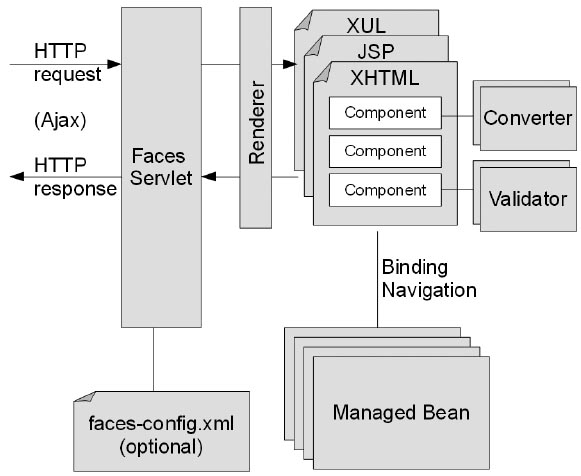
\includegraphics[width=\textwidth]{jsf_mvc}
\caption{Arquitetura JSF}
\label{fig1}
\end{figure}


\begin{figure}
\centering
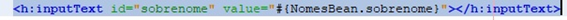
\includegraphics[width=\textwidth]{render1}
\caption{Renderers 1}
\label{fig2}
\end{figure}


\begin{figure}
\centering
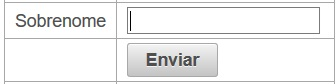
\includegraphics[width=\textwidth]{render2}
\caption{Renderers 2}
\label{fig3}
\end{figure}


\begin{figure}
\centering
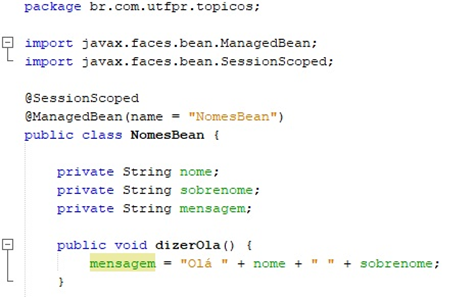
\includegraphics[width=\textwidth]{managed_bean}
\caption{Exemplo de classe managed bean}
\label{fig4}
\end{figure}


\begin{figure}
\centering
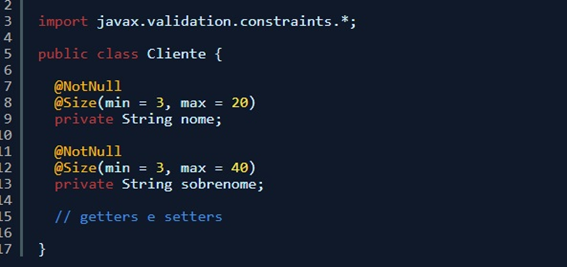
\includegraphics[width=\textwidth]{bean_validation}
\caption{Exemplo de código utilizando o Validation}
\label{fig5}
\end{figure}


\begin{figure}
	\centering
	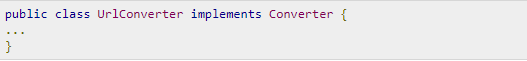
\includegraphics[width=\textwidth]{converters3}
	\caption{Exemplo implementação classe converter}
	\label{fig6}
\end{figure}


\begin{figure}
	\centering
	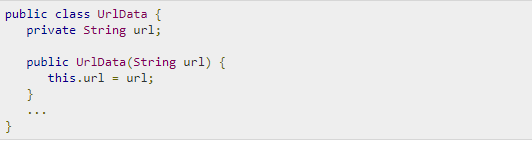
\includegraphics[width=\textwidth]{converters4}
	\caption{Exemplo de classe para armazenar dados}
	\label{fig7}
\end{figure}


\begin{figure}
	\centering
	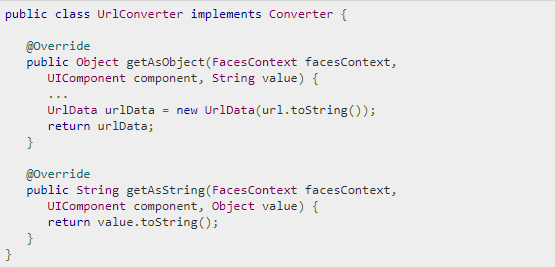
\includegraphics[width=\textwidth]{converters5}
	\caption{Exemplo utilização de método}
	\label{fig8}
\end{figure}


\begin{figure}
	\centering
	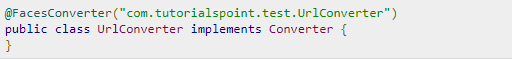
\includegraphics[width=\textwidth]{converters6}
	\caption{Exemplo de registro do converter}
	\label{fig9}
\end{figure}


\begin{figure}
	\centering
	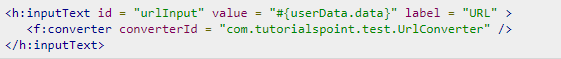
\includegraphics[width=\textwidth]{converters7}
	\caption{Exemplo de uso do converter}
	\label{fig10}
\end{figure}


\begin{figure}
	\centering
	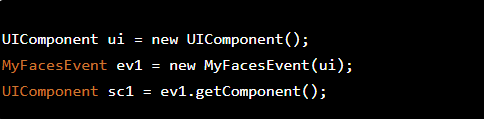
\includegraphics[width=\textwidth]{event1}
	\caption{Exemplo chamada de evento}
	\label{fig11}
\end{figure}


\begin{figure}
	\centering
	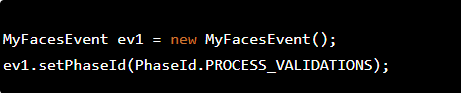
\includegraphics[width=\textwidth]{event2}
	\caption{No código acima, os eventos ocorrerão no final da fase de validação do processo}
	\label{fig12}
\end{figure}


\begin{figure}
	\centering
	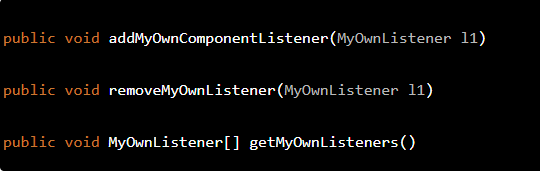
\includegraphics[width=\textwidth]{listener1}
	\caption{Os métodos acima devem ser definidos para registrar a classe do listener}
	\label{fig13}
\end{figure}


\begin{figure}
	\centering
	
\includegraphics[width=\textwidth]{navigation1}
	\caption{Exemplo de resultado na página JSF}
	\label{fig14}
\end{figure}


\begin{figure}
	\centering
	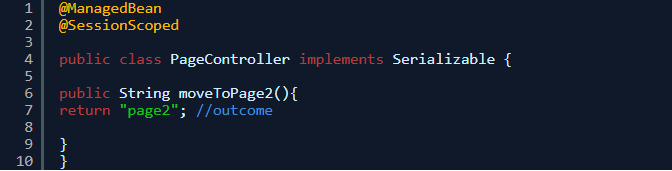
\includegraphics[width=\textwidth]{navigation2}
	\caption{Resultado em um managed bean}
	\label{fig15}
\end{figure}


\begin{figure}
	\centering
	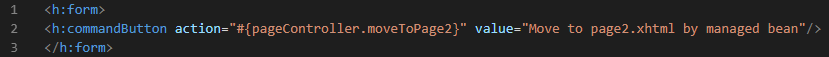
\includegraphics[width=\textwidth]{navigation3}
	\caption{Exemplo usando "method expression"}
	\label{fig16}
\end{figure}






\end{document}